% HIEU Model Flowchart - Simplified Version
\documentclass[tikz,border=10pt]{standalone}
\usepackage{tikz}
\usetikzlibrary{shapes.geometric, arrows.meta, positioning, fit, backgrounds, calc}
\usepackage{amsmath}
\usepackage{amssymb}

% Define colors
\definecolor{inputcolor}{RGB}{187, 222, 251}
\definecolor{contextcolor}{RGB}{255, 224, 178}
\definecolor{predcolor}{RGB}{200, 230, 201}
\definecolor{outputcolor}{RGB}{225, 190, 231}
\definecolor{regimecolor}{RGB}{239, 154, 154}
\definecolor{graphcolor}{RGB}{165, 214, 167}
\definecolor{freqcolor}{RGB}{255, 224, 130}
\definecolor{hypercolor}{RGB}{206, 147, 216}
\definecolor{corecolor}{RGB}{144, 202, 249}

\begin{document}
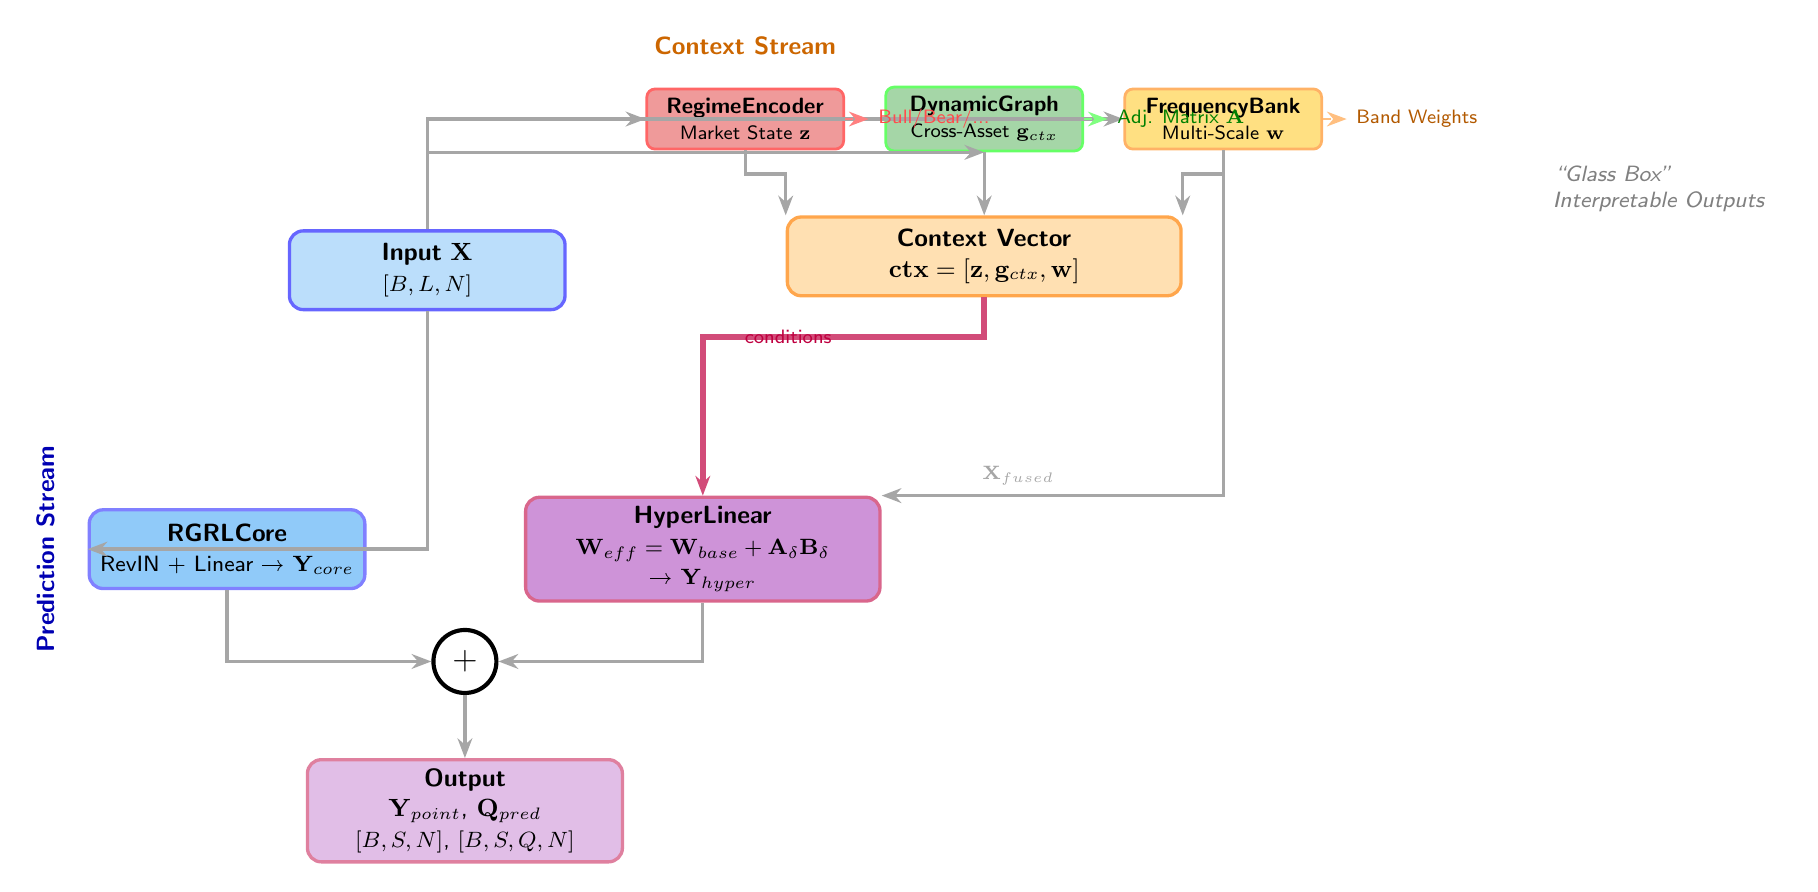
\begin{tikzpicture}[
    node distance=0.6cm and 1.5cm,
    >={Stealth[length=2.5mm]},
    box/.style={rectangle, draw, rounded corners=5pt, minimum width=3.5cm, minimum height=1cm, align=center, font=\sffamily\small, line width=1.2pt},
    smallbox/.style={rectangle, draw, rounded corners=3pt, minimum width=2.5cm, minimum height=0.7cm, align=center, font=\sffamily\footnotesize, line width=1pt},
    arrow/.style={->, line width=1.2pt, gray!70},
    thickarrow/.style={->, line width=2pt},
    label/.style={font=\sffamily\scriptsize, text=gray}
]

% ========== INPUT ==========
\node[box, fill=inputcolor, draw=blue!60] (input) {
    \textbf{Input} $\mathbf{X}$\\
    {\footnotesize $[B, L, N]$}
};

% ========== CONTEXT STREAM ==========
\node[smallbox, fill=regimecolor, draw=red!60, above right=1cm and 1cm of input] (regime) {
    \textbf{RegimeEncoder}\\
    {\scriptsize Market State $\mathbf{z}$}
};

\node[smallbox, fill=graphcolor, draw=green!60, right=0.5cm of regime] (graph) {
    \textbf{DynamicGraph}\\
    {\scriptsize Cross-Asset $\mathbf{g}_{ctx}$}
};

\node[smallbox, fill=freqcolor, draw=orange!60, right=0.5cm of graph] (freq) {
    \textbf{FrequencyBank}\\
    {\scriptsize Multi-Scale $\mathbf{w}$}
};

% Context concat
\node[box, fill=contextcolor, draw=orange!70, below=0.8cm of graph, minimum width=5cm] (ctx) {
    \textbf{Context Vector}\\
    $\mathbf{ctx} = [\mathbf{z}, \mathbf{g}_{ctx}, \mathbf{w}]$
};

% ========== PREDICTION STREAM ==========
\node[box, fill=corecolor, draw=blue!50, below left=2.5cm and -1cm of input] (core) {
    \textbf{RGRLCore}\\
    {\footnotesize RevIN + Linear → $\mathbf{Y}_{core}$}
};

\node[box, fill=hypercolor, draw=purple!60, right=2cm of core, minimum width=4.5cm] (hyper) {
    \textbf{HyperLinear}\\
    {\footnotesize $\mathbf{W}_{eff} = \mathbf{W}_{base} + \mathbf{A}_\delta\mathbf{B}_\delta$}\\
    {\footnotesize → $\mathbf{Y}_{hyper}$}
};

% Addition node
\node[circle, draw, fill=white, line width=1.5pt, minimum size=0.8cm, below=1cm of $(core)!0.5!(hyper)$] (add) {\large $+$};

% ========== OUTPUT ==========
\node[box, fill=outputcolor, draw=purple!50, below=0.8cm of add, minimum width=4cm] (output) {
    \textbf{Output}\\
    $\mathbf{Y}_{point}$, $\mathbf{Q}_{pred}$\\
    {\footnotesize $[B, S, N]$, $[B, S, Q, N]$}
};

% ========== ARROWS ==========
% Input to context modules
\draw[arrow] (input.north) |- (regime.west);
\draw[arrow] (input.north) |- (graph.south);
\draw[arrow] (input.north) |- (freq.west);

% Context modules to concat
\draw[arrow] (regime.south) -- ++(0,-0.3) -| (ctx.north west);
\draw[arrow] (graph.south) -- (ctx.north);
\draw[arrow] (freq.south) -- ++(0,-0.3) -| (ctx.north east);

% Input to prediction stream
\draw[arrow] (input.south) |- (core.west);
\draw[arrow] (freq.south) |- node[pos=0.8, above, font=\scriptsize] {$\mathbf{X}_{fused}$} (hyper.north east);

% Context to HyperLinear
\draw[thickarrow, purple!70] (ctx.south) -- ++(0,-0.5) -| node[pos=0.25, left, font=\scriptsize\sffamily, text=purple] {conditions} (hyper.north);

% To addition
\draw[arrow] (core.south) |- (add.west);
\draw[arrow] (hyper.south) |- (add.east);

% To output
\draw[arrow] (add.south) -- (output.north);

% ========== LABELS ==========
\node[above=0.3cm of regime, font=\sffamily\small\bfseries, text=orange!80!black] {Context Stream};
\node[left=0.3cm of core, font=\sffamily\small\bfseries, text=blue!70!black, rotate=90, anchor=south] {Prediction Stream};

% ========== INTERPRETABILITY ANNOTATIONS ==========
\node[right=0.3cm of regime, font=\scriptsize\sffamily, text=red!70] (r1) {Bull/Bear/...};
\node[right=0.3cm of graph, font=\scriptsize\sffamily, text=green!50!black] (r2) {Adj. Matrix $\mathbf{A}$};
\node[right=0.3cm of freq, font=\scriptsize\sffamily, text=orange!70!black] (r3) {Band Weights};

\draw[->, dashed, red!50, line width=0.8pt] (regime.east) -- (r1.west);
\draw[->, dashed, green!50, line width=0.8pt] (graph.east) -- (r2.west);
\draw[->, dashed, orange!50, line width=0.8pt] (freq.east) -- (r3.west);

% Glass box annotation
\node[below right=0.2cm and 0.5cm of r3, font=\sffamily\footnotesize\itshape, text=gray] {
    \begin{tabular}{l}
    ``Glass Box''\\
    Interpretable Outputs
    \end{tabular}
};

\end{tikzpicture}
\end{document}
